\documentclass[a4paper]{article}
\usepackage{graphicx}
\usepackage{hyperref}
\usepackage{parskip}
\usepackage[a4paper]{geometry}

\begin{document}

\begin{titlepage}
\vspace{10em}
\centering
{\LARGE Amazon Picking Challenge 2016}

\hrule

{\Huge Team Delft software architecture}

\today

\hrule

\tableofcontents

\vfill
\end{titlepage}

\section{Introduction}
The purpose of this document is to define the high level components of the Team Delft software system,
and more importantly the interfaces between these components.

Keep in mind that this document is not set in stone.
If changes are needed please discuss with the rest of the team and the document will be updated.

The global design of the system consists of 7 components:

\begin{itemize}
\item Coordinator
\item Vision
\item Camera driver
\item Grasp planner
\item Placement planner
\item Trajectory planner
\item Robot driver
\end{itemize}

An overview of this design is shown in \autoref{fig:global-architecture}.

Each component internally can consist of multiple subcomponents.
For the purpose of this document, these subcomponents are considered implementation details.
They are not relevant to the other high level components, so they are not outlined here.

There may also be some small components missing from this design.
For example for moving the camera if it is attached to a dedicated 2D frame.
However, these should not affect the interfaces described in this document.

Also note that these components do not necessarily correspond to ROS nodes.
It is possible that components will be split in multiple nodes,
or that some components will be combined in a single node.

\begin{figure}[hbtp]
	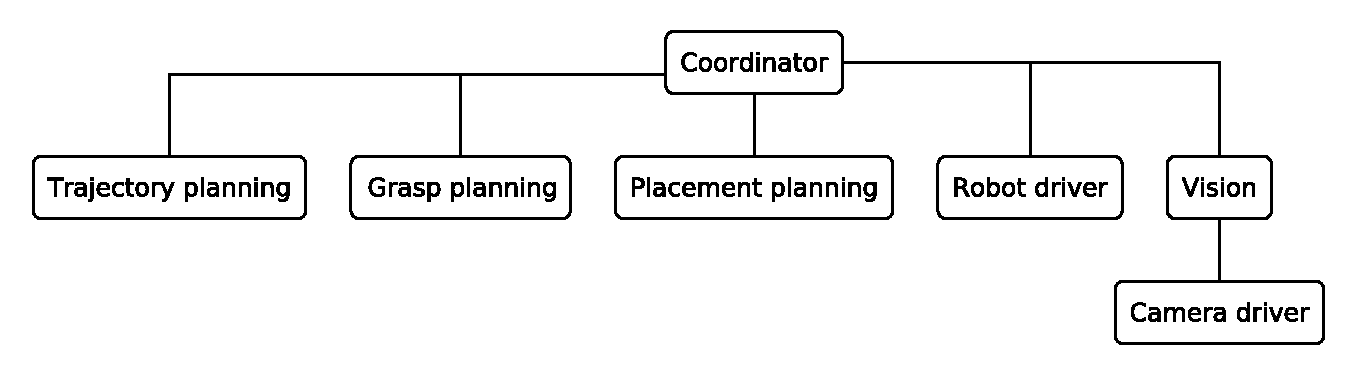
\includegraphics[width=\textwidth]{figures/global-architecture}
\caption{Global software architecture}
\label{fig:global-architecture}
\end{figure}


\section{Components}

\subsection{Coordinator}
The coordinator is responsible for deciding what to do when.
It will also monitor the status of each task and respond accordingly if tasks fail, succeed or hang.

In general, other components should not talk to each other directly but wait for instructions from the coordinator.
One exception to this is vision, which in the current design communicates directly with the camera driver.

The coordinator does not expose interfaces to other components.


\subsection{Vision}
The vision component performs the vision tasks.

\subsubsection*{Bin scanning}
One task for the vision component is to scan a bin and return the visible contents.
For this task, the vision component will be informed which items should be present within the bin.
The exact interface is as follows:

\begin{tabular}{| l | l |}
\hline
\multicolumn{2}{| l |}{Input parameters} \\
\hline
expected\_objects & A list of expected objects in the tote/bin. \\
\hline
\multicolumn{2}{ l }{} \\
\hline
\multicolumn{2}{| l |}{Return result} \\
\hline
found\_objects  & A list of found objects, including the type and pose of each object. \\
\hline
\end{tabular}

\subsection*{Tote scanning}
A second task for the vision component is to scan the tote and return the visible contents.
Again, the vision component will be informed what items should be present in the tote.
The interface is exactly the same as for the previous task:

The interface for the calibration is different:

\begin{tabular}{| l | l |}
\hline
\multicolumn{2}{| l |}{Input parameters} \\
\hline
expected\_objects & A list of expected objects in the tote/bin. \\
\hline
\multicolumn{2}{ l }{} \\
\hline
\multicolumn{2}{| l |}{Return result} \\
\hline
found\_objects  & A list of found objects, including the type and pose of each object. \\
\hline
\end{tabular}

\subsubsection*{Bin empty place scanning}
In some cases, items must also be placed back in bins.
This is obvious for the stowing challenge,
but it may also occur during the picking challenge if the desired item could not be found.
To facilitate this, the vision component has an interface for detecting empty space within a bin.

\begin{tabular}{| l | l |}
\hline
\multicolumn{2}{| l |}{Return result} \\
\hline
empty\_spaces  & A list of detected empty spaces,
each space being defined as a box where no other objects are present. \\
\hline
\end{tabular}

\subsubsection*{Calibration}
The vision sensors must also be calibrated with respect to the robot.
To this end, the vision component has a third interface which will detect a known calibration pattern.
Since the pattern is already known, there are no input parameters.
The only output parameter is the detected pose of the calibration pattern:

\begin{tabular}{| l | l |}
\hline
\multicolumn{2}{| l |}{Return result} \\
\hline
pose  & The pose of the detected calibration pattern. \\
\hline
\end{tabular}


\subsection{Camera driver}
The camera driver is responsible for grabbing sensor data.
It provides a single interface for acquiring image data.

\subsubsection*{Image acquisition}
The driver will use a pull model where a new image is requested when needed,
rather than the camera continuously streaming images.
The interface is as follows:

\begin{tabular}{| l | l |}
\hline
\multicolumn{2}{| l |}{Return result} \\
\hline
color  & The recorded color image, synchronized with the other data. \\
depth  & The recorded depth image, synchronized with the other data. \\
cloud  & The recorded point cloud, synchronized with the other data. \\
\hline
\end{tabular}

The returned data must be synchronized, meaning that the images and point cloud were all recorded at the same moment.

Note that unneeded information can be removed form the return result once the vision algorithms are decided.


\subsection{Grasp planner}
The grasp planner will determine a grasp pose for the robot end-effector given the type and pose of an object to grasp.

\subsubsection*{Shelf grasping}
The interface for planning a grasp pose for an object in a shelf is as follows:

\begin{tabular}{| l | l |}
\hline
\multicolumn{2}{| l |}{Input parameters} \\
\hline
object\_type & The type of the object to grasp. \\
pose         & The pose of the object to grasp. \\
\hline
\multicolumn{2}{ l }{} \\
\hline
\multicolumn{2}{| l |}{Return result} \\
\hline
pose & The grasp pose for the end-effector. \\
\hline
\end{tabular}

\subsubsection*{Tote grasping}
The interface for planning a grasp pose for an object in the tote is as follows:

\begin{tabular}{| l | l |}
\hline
\multicolumn{2}{| l |}{Input parameters} \\
\hline
object\_type & The type of the object to grasp. \\
pose         & The pose of the object to grasp. \\
\hline
\multicolumn{2}{ l }{} \\
\hline
\multicolumn{2}{| l |}{Return result} \\
\hline
pose & The grasp pose for the end-effector. \\
\hline
\end{tabular}


\subsection{Placement planning}
The placement planner will determine a placement pose for the robot end-effector
given the type of object and list of areas where it could be placed.

\subsubsection*{Bin object placing}
The interface for planning a placement pose for an object in a shelf is as follows:

\begin{tabular}{| l | l |}
\hline
\multicolumn{2}{| l |}{Input parameters} \\
\hline
object\_type     & The type of the grasped object. \\
pose             & The pose of the grasped object relative to the end-effector. \\
available\_space & A list of boxes of empty space where the object can be placed. \\
\hline
\multicolumn{2}{ l }{} \\
\hline
\multicolumn{2}{| l |}{Return result} \\
\hline
pose & The placement pose for the end-effector. \\
\hline
\end{tabular}

The input pose parameter is the pose of the object within the end-effector.
It may be an estimated pose if it can not be measured.


\subsection{Trajectory planner}
The trajectory planner will plan trajectories for the robot.
There are a number of different trajectories to be planned.
In general though, each trajectory is defined by what action is being performed,
the start configuration of the robot and the end configuration of the robot.
As such, each of the different planning tasks will use the same interface.

The different trajectories that must be planned are:
\begin{itemize}
	\item The shelf approach trajectory.
	\item The shelf retreat trajectory.
	\item The tote approach trajectory.
	\item The tote retreat trajectory.
\end{itemize}

These trajectories must be planned for the picking challenge but also for the stowing challenge.
That gives a total of 8 trajectories that can be planned.

If an eye-in-hand configuration is chosen,
more trajectories are added for positioning the camera with the robot.


\subsubsection*{Trajectory planning}
Each trajectory that can be planned will use the following interface:

\begin{tabular}{| l | l |}
\hline
\multicolumn{2}{| l |}{Input parameters} \\
\hline
start\_configuration & The start configuration of the robot in joint space. \\
end\_pose            & The desired end pose for the end effector. \\
\hline
\multicolumn{2}{ l }{} \\
\hline
\multicolumn{2}{| l |}{Return result} \\
\hline
trajectory & The planned trajectory. \\
\hline
\end{tabular}

As with the grasp planning,
if more information is needed for the planning it must be added to the input parameters.

\end{document}
